\pagenumbering{arabic} % start using arabic page numbers


% Plagerism checker https://www.quetext.com/


\chapter{Background}\label{chap:Background}

\section{Introduction}

\begin{figure}[b]
	\centering
	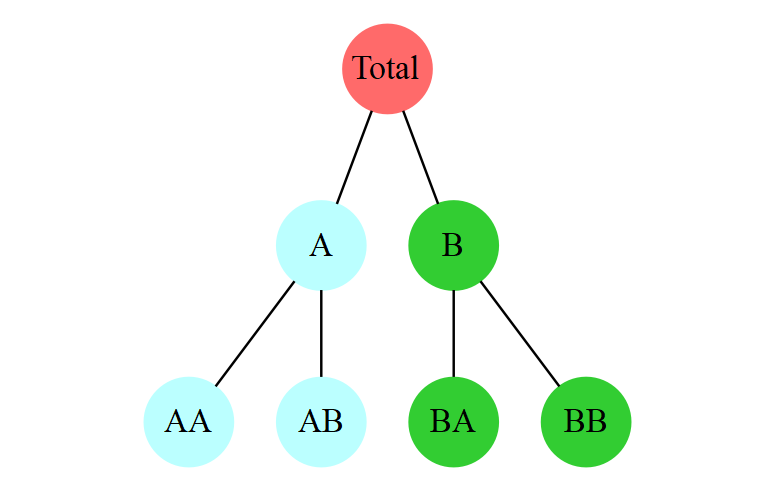
\includegraphics[width=0.4\linewidth]{Figures/treesimple}
	\caption{A two level hierarchical tree diagram}
	\label{fig:htstree}
\end{figure}

Large datasets often have a hierarchical structure (as seen in figure~\ref{fig:htstree}), in other words, data may organised into a tree-like structure, where broader categories with higher hierarchy may disaggregate into smaller categories with lower hierarchy. Vice versa, smaller categories with lower hierarchy may aggregate into broader categories with higher hierarchy. In a clinical trial, Adverse Events (AEs) caused by treatment drugs can be aggregate into body systems that are associated with AEs, thus creating a 2-level hierarchical structure. An example of a study considering such hierarchical structure is \cite{berry2004}, the study considers the probabilities of treatment drug cause an AEs and found significant differences in results between solo ( with each category independently modelled) and Hierarchical Bayesian Model (HBM) at the bottom level of the hierarchy, and suggested that the HBM could be a solution to the multiplicity problem found in large datasets. Similarly, disease diagnoses also have a complex, hierarchical structure, where different categories of diagnoses aggregated into broader categories. Standard such as International Statistical Classification of Diseases and Related Health Problems (ICD)\citep{WHO2019} are used to code for and organise disease diagnosis into a hierarchical structure. Information about ICD diagnoses often included in hospital archives for research and managerial purposes. Note that ICD diagnosis is not the equivalent to original diagnosis by doctors, descriptions of diagnoses can vary doctor to doctor, it is non-consistent and unorganised at first, this diagnosis is then classified into standard ICD diagnosis which is standard, organised and has clear hierarchical properties. 

%A hierarchical structure is also frequently seen in genetics data, Gene Ontology (GO) groups different genes into a multi-domain hierarchical network \citep{GO2007}, which is a representation of genetic relationship and network of significant GO categories often serve as a basis for genetic analyses.

\newpara 

We are interested in whether modelling the full hierarchy gives a better understanding of anomalies compares to modelling each category independently one level at a time. When modelling too broad a category, individual variations could be missed; when model too narrow a category, there may be too little data with non-significance. Vital information are likely be lost if we only consider one level at a time and if the information doe not situated at the level considered, so why not consider every possible level? A hierarchical model retains information from all level of the hierarchy and may provide better predictions compare to standard models that do not implicate the hierarchical structure of the data. The purpose of this research thesis is to investigate the use of Hierarchical Bayesian Models (HBM) as a possible approach for the detection of anomalies from hierarchical datasets. In this chapter, we describe examples of where these issues arise, and layout the technical background for our methods. 

%------------------------------------------------------------------------------------------

\section{Emergency Department Congestion}

While the world population continues to grow and age at an unprecedented rate, public healthcare system all over the world are expected to experience an increasing number of situations where a massive influx of patients overwhelms the current healthcare capability and in which congestion occur \citep{ morley2018emergency, wong2010understanding}. Other similar terms used to describe this situation include bottleneck and overcrowding. Congestion is shown to have negative influences on both patient and hospital staff, studies \citep{chambers2016burnout, khare2009adding, salway2017emergency} suggest that congestion is positively associated with adverse outcomes such as patient waiting time, short term patient mortality, medical errors, and professional burnout in hospital staff; therefore we would want to avoid or reduce the possibility of occurrence of congestions. Congestion seriously challenges the capability of public healthcare system worldwide and are becoming increasingly burdensome in many locations, and efforts from healthcare systems are struggling to kept pace with increasing demands. The overall consensus is that the demand from the ageing population is one of the major contributing factors to the current crisis, and the factor of ageing is unlikely to improve by time \citep{bayley2005financial, cornwall2004impact, wong2010understanding}. For instance, the national population projections by Stats New Zealand (2016) predicts a constant increasing trend in older (age 65 +) populations and show no sign of slowing down, so the problem of congestion in New Zealand in another hand, will most likely to correspond to this and worsen. 
%http://archive.stats.govt.nz/browse_for_stats/population/estimates_and_projections/NationalPopulationProjections_HOTP2016.aspx

\newpara

Shortage of staff for public healthcare services has been a prominent issue ever since a decade of decrease in the proportion of healthcare funding and deficit for the public health system in New Zealand \citep{akoorie2018, WB2019}. Due to limitations with medical material and human resources, hospital staff often had to operate at full capacity and are therefore under tremendous stress. Studies have shown that under-staffing is one of the key factors that contribute to the high prevalence of professional burnout in New Zealand’s public hospital senior medical workforce \citep{chambers2016burnout}. Described as “erosion of the soul” by Doctor Len Gabbard, in an article by \cite{HemOnc2008}, professional burnout is a term used in industry research that refers to a sense of emotional exhaustion, negative attitudes and sense of incompetence that often lead to reduced work effectiveness \citep{paterson2011professional}. Therefore burnout has negative impacts and to reduce this; we would need to optimise the way the hospital operates.  

\newpara

Due to the increasing patient influx and understaffing, some Emergency Department (ED) in the country struggled to cope with increasing patient arrivals; this is reflected from unacceptable delays before patients are admitted to hospital, transferred or sent home. Patient delay is a direct result of triage strategy \citep{MoH19triage} utilised by ED if congestion of patients occurs. When there is not enough staff to cope with patient demand, the patient at a higher triage is given a priority for treatment (higher the triage level, the more critical patient is believed to be). However, a critical flaw of the current strategy is that if congestion does not get resolved, and lots of patients require immediate treatment, a patient that is evaluated to be less urgent often gets delay after delay. In theory, a patient can be delayed for infinity if he is unfortunate enough, and the chance of further complication developing during the waiting period will only rise at every second of the clock ticking by. 

\newpara

A tragic case happened in New Zealand, back in 2015, where a woman in Wellington died after 12 hours of delay and ignorance in emergency medical service \citep{southland2015}. The news reported that \textit{“The emergency department was stretched by an influx of patient which lead to congestion and overcrowding”}, so ED staff had decided that the patient was not in an immediately life-threatening situation and decided to apply the triage strategy and therefore delayed medical service. What supposed to be a 30-minute delay had turned into more than an hour, and over the last 12 hour of the patient's life, ED staff failed to provide adequate monitor and care, which was believed to have contributed to the patient’s untimely demise.  It breaks your heart when you hear such case happening and you cannot stop wondering, what if the patient was treated in time? 

\section{Motivation}

Located at the start of the healthcare pathway \citep{MoH19pathway}, the Emergency Department (ED) and other forms of emergency health care are feeling tremendous pressure from increasing healthcare demands. Compare to primary healthcare, emergency healthcare is a 24/7 operating service characterised with unscheduled visits, and mostly deals with critical conditions that need immediate attention \citep{MoH19ed, MoH19primary}, therefore ED frequently encounters an influx of unanticipated emergencies such as major traffic accident, mass food poisoning and disease outbreaks. Unfortunately, due to limited and often diminishing resources, public healthcare facilities often had to operate at near full capacity to reduce operation costs \citep{salway2017emergency}, and this leaves a very small buffer zone to deal with abnormally high arrivals, so it is quite safe to suggest that ED staffs are underprepared for congestion.    

\newpara

The congestion crisis in the New Zealand healthcare service stood well recognised by the academic community, and there is a substantial amount of recent and ongoing research that aims at providing alternative operational strategies. For instance, \citet{adam2018} is currently working on simulations of Auckland city hospital’s Emergency Department with Pod model, where doctors form small cross-functional and multidisciplinary teams. Experimental trials had taken place at the Auckland city hospital during December 2018 - January 2019 to evaluate the effectiveness of Pods strategy compare to the precedent triage strategy. Another interesting study is a study by \citet{Cleland2018} that looked at developing algorithms to optimise staff rostering, compares to precedent; his algorithm found many new ways staff rostering can be improved and thus could improve the operational effectiveness of hospital. As we can see, we do have people approaching the problem in various ways. 

\newpara

For this thesis, we want to approach the problem of congestion in public hospitals through the perspective of Healthcare Logistics. As Prof.Dr. Stephan Nickle from Karlsruhe Institute of Technology (KIT) Quoted during the 2018 Operations Research Society of New Zealand (ORSNA) conference \citep{Nickle2018}, \textit{“Healthcare Logistics is all about the robustness and smoothness of the operation”}, what we want is stability and predictability of the operation, even if on paper we have a high efficiency, it is no good if this efficiency is often compromised. ED congestion often occurs during the periods of abnormal arrivals when the max capacity is overwhelmed; therefore, a success prediction/anticipation of such abnormal arrivals could provide valuable insight for operational planning and management. Public hospital was supposedly prepared, medical facilities continually being built, medical supplies prepared in advance, and staff were recruited base on predictions from historical mean arrivals. It would make sense to the thought that the public health system was well prepared, right? However, why are we still seeing congestions? Well, what happened is that the public health system had well prepared for normality, but has overlooked instances of abnormality. Lots of operational and logistics planning and based on mean values, however, means does not contain information about abnormality. To the inconvenience of everybody involved, congestion occurs during abnormal arrival events.

\newpara

If we could make sense of and make informed predictions about abnormal patient arrivals, it would provide helpfulness to the planning and management of the public healthcare system. Doctors can transfer, and medical supplies can be in preparation as soon as there is enough evidence suggesting an abnormal event is or will be happening. With better preparation and faster response to abnormal patient arrivals, the problem of congestion could be alleviated, and benefit both patient and healthcare staff. For patients, a shorter delay waiting period will increase the quality and timeliness of the medical service provided and reduce the risk of further complications during the wait. Moreover, for doctors, more preparedness should reduce professional burnout and increase efficiency \citep{chambers2016burnout, khare2009adding}. For this thesis, a strong emphasis is placed on modelling anomaly detection for patient arrivals, in the hopes of that extension on the understanding of anomalous arrival events could be made, and provide information for theoretical and real-life implications. 

%------------------------------------------------------------------------------------------

\section{Anomaly Detection} \label{chap:anom}

Anomaly detection refers to the field of studies of finding patterns in data that does not conform to the expectation, or that is out of normality. Studies of anomaly can trace back to the 19th century; an example is that in 1887, F. Y. Edgeworth a lecturer from King’s College, London wrote about what he termed as discordant observations, observations which \textit{“present the appearance of differencing in respect of their law of frequency from other observation with which they are combined”} \citep{edgeworth1887xli}. The term anomaly is quite similar to the term outlier, which is defined by “A data point that differs significantly from other observations” \citep{grubbs1969procedures}, and these two terms often used interchangeably. However, the term anomaly has a stronger contextual connection to the application side of the statistics, the wording itself literally meant, an event that is not of normal circumstance. 

\newpara

Anomaly detection found extensive application in fields such as cyber-security, finance, and healthcare. The reason why anomaly is catching so much research interest is that it often strongly associate with and directly translates into the occurrence of harmful situations and events in dynamic environments \citep{chandola2009anomaly, LaRosa2018}. The classic example of anomaly detection often described by Data scientists is the application of intrusion detection systems that are triggered by anomalies that are believed to be indicators of cyber-attacks. An indicator such as abnormally high website visits could be an indication of an HTTP POST attack, where the website processing capacity is overwhelmed, or maybe illegal data scraping, where private information is processed and exported from a website \citep{patcha2007overview, Target2018}. Due to growing concerns of potential bioterrorism attack following the anthrax letters attacks to various government officials during 2001, the US had been invested in the field of Biosurveillance in preparation for a potential bioterrorism attack \citep{grundmann2014current}. Therefore a substantial amount of research regarding population-level anomaly detection is available. For instance, back in 2003, \citep{wong2003bayesian} has presented the WSARE 3.0 algorithm, which stands for "What's Strange About Recent Events, version 3” for the detection of disease outbreaks in the US. Also, in \textit{Intelligence and Security Informatics: Biosurveillance}, a text published in 2007, \citet{bauer2007high} suggest the need of rapid data processing for anomaly detection to meet the increasing demand to disease surveillance at a population level. Their idea foreshadowed the recent rise in popularity of online streaming data systems that collect data from multiple sources continuously and provide statistical results right with each update.  

\newpara

For the case of patient arrivals, researchers often take an interest in time series data. That is, a continuing set of data that is recorded over specific time intervals \citep{das1994time}. If information about the time of each patient visit is available, it can be counted to give a time series data over time-periods, such as the number of patient arrivals per day. From the perspective of time series data, there are several important types of anomalies to be considered.  The first and most straightforward type is point anomalies, where a single time-period is anomalous. For example, traffic of a website may spike during a single night, when the website is under cyber-attack. The second and more complex type is period anomalies, where a continuing series of time-periods is anomalous. For example, the average daily spending during the Christmas period (let us say, the days between 1 December to 31 December) is expected to be much higher when compared to the average usual daily spending in other time frames. The last type, Contextual anomalies, where the occurrence of the anomalous time-period is believed to be context-specific. For example, the Admission rates for Emergency department patients may spike on any given day, when there is a mass injury event such as major car crashes \citep{chandola2009anomaly}. In this thesis, we want to focus on just the point anomaly, because other forms of anomalies are very context-specific and hard to perform in simulated settings. 

\newpara

There are many ways to decide whether a point or a pattern is abnormal and deviate from the expected; the most straightforward and often used approach is to set up value as thresholds, and then anomalies can be detected simply by raising alarms for observing values beyond the threshold (figure~\ref{fig:anomaly}).

\begin{figure}[h]
	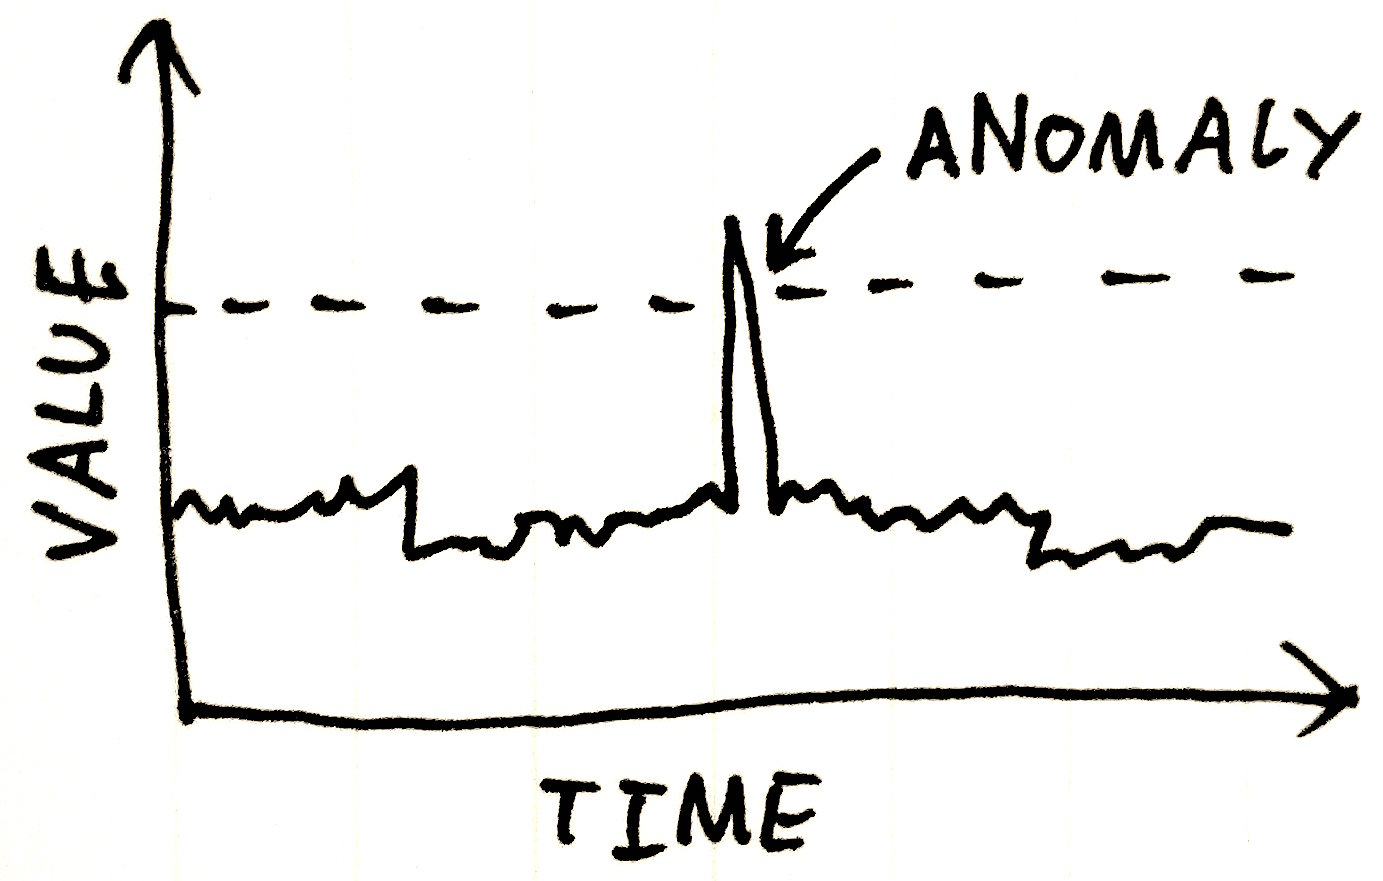
\includegraphics[width=47mm]{Figures/external/simple_anomaly}
	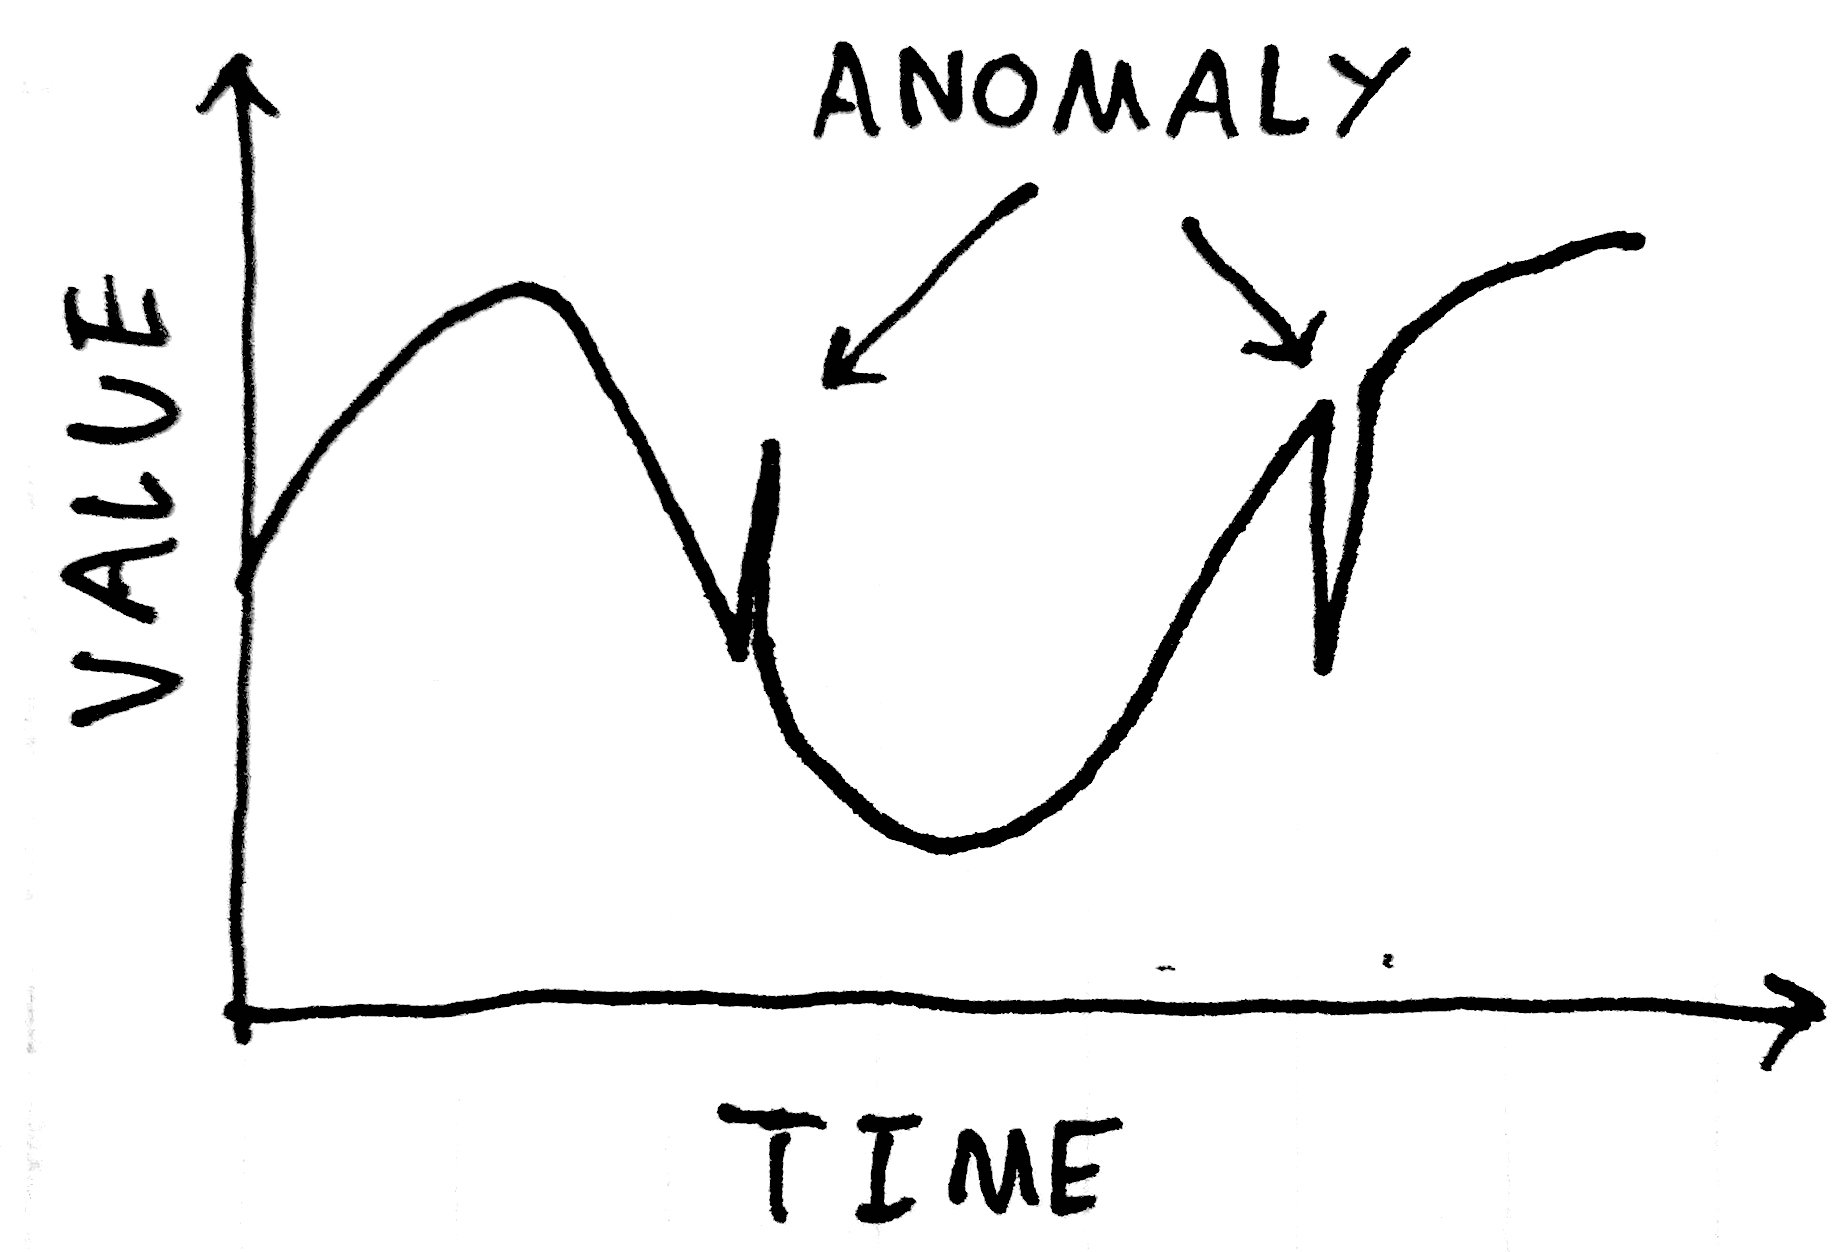
\includegraphics[width=47mm]{Figures/external/harder_anomaly}
	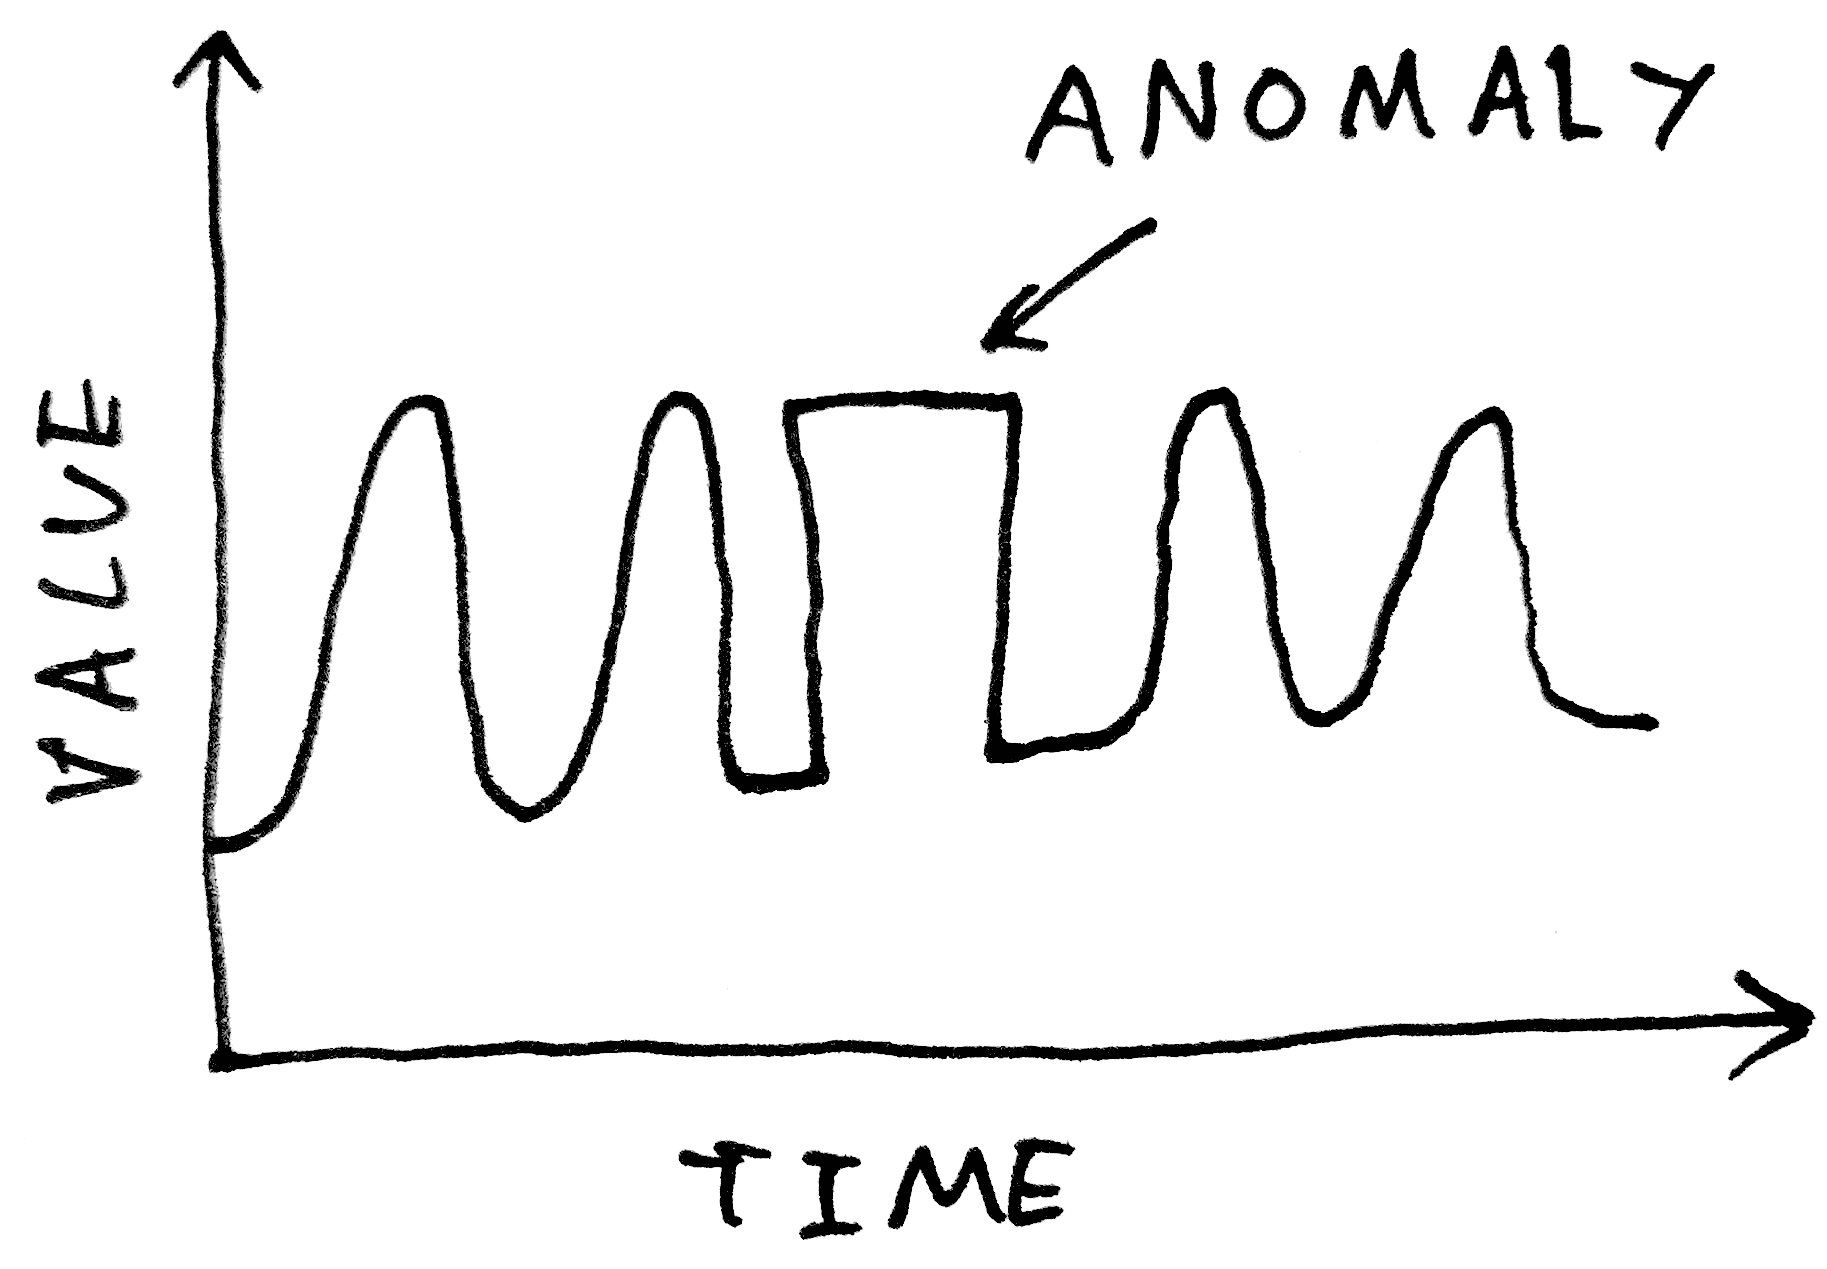
\includegraphics[width=47mm]{Figures/external/really_hard_anomaly}
	\caption{Anomaly Visualisation from \citet{Rahtz2015}}
	\label{fig:anomaly}
\end{figure}

\citet{wong2003bayesian} considered the threshold approach and proposed the standard algorithm. Their anomaly detector considers the mean $\mu$ and variance $\sigma$of the total number of records on each day, and used algorithm shown in equation~\ref{equ:threshold} to calculate a threshold, For the algorithm $\Phi^{-1}$ is the inverse to the cumulative distribution function of a standard normal with an user-defined p-value. If the aggregate daily counts of health care data exceed this threshold during the evaluation period, an alarm can raise. 

\begin{equation}\label{equ:threshold}
\begin{aligned}
threshold = \mu + \sigma * \Phi^{-1}(1-\dfrac{\text{p-value}}{2})
\end{aligned}
\end{equation}


We propose a simpler algorithm that approaches the threshold set up from a more practical point of view, rather than a theoretical statistical value such as $\Phi^{-1}$ used by \citet{wong2003bayesian}. We want to create two values called load ($\mu$) and capacity ($C$), $C$ are the full treatment capacity in terms of absolute value of a department, and $\mu$ the average number of capacity being occupied and utilised. In theory, $\mu$ and $C$ could be generated from hospital records such as the number of hospital beds occupied, the number of doctors that are currently treating a patient and not available for another patient in a short notice, and any other available measures of hospital operational capacities. $\mu$ over $C$ gives a load fraction, which are referred as capacity in terms of percentage. If we assume that the healthcare system is expected to be operating at a capacity value ($k$) of 0.8, it would mean that on average, 80\% of total possible treatment resource during a specific period is utilised. 

\begin{equation}\label{equ:threshold2}
\begin{aligned}
k = \mu C^{-1}
\end{aligned}
\end{equation}

In simple terms threshold would just be the full capacity $C$, however we want to compare between low and high capacity departments so capacity $k$ are used in our study. So if a hospital department on average treats 100 patient per day, and this department is considered to be operate at 80\% capacity, the threshold would be $100 \times 0.8^{-1} = 100 \times 1.25 = 125$. The idea is that when we reached the threshold, it would mean that the healthcare capacity of the period had reached 100\%, and there is no more capacity for more patients, and in theory, this is when congestion would for definitely, occur. Instead of only considering operating cost, an ideal operating percentage should be relatively high to reduce operating cost, and have gives a low chance of overcapacity due to the anomalous event. Following up on the idea by Stephan Nickle, mentioned in the previous section, we propose that increasing the operational capacity without considering anomalous events could jeopardise the smoothness of operation, and cause even more loss of operating efficiency due to increased probability congestions. 

\newpara

To create an alarm system that raises alarms for hospital congestion, we could apply a threshold on to patient arrivals, with every increase in the number of patients arrived, it would become more likely that a threshold can exceed. However, the catch is that we should also incorporate external information such as the number of bed available instead of only considering with numerical probability. How could we possibly know if we have reached the full hospital capacity if we only consider the number of beds used, without knowledge of the number of total beds available? With only information about observed arrivals, we could work out the likelihood of observing specific arrival numbers, but this outcome does not make any practical sense by itself. Information is one of the reasons why the standard algorithm proposed by \citet{wong2003bayesian} although performed excellently, still seem weak for practical applications. The standard algorithm considers the threshold as the im-probability from the data structure and does not consider what determines the threshold, the ability or the capacity for hospitals to treat patients. A particular statistical inference approach does incorporate external information and solves this problem, as people might have guessed already, Bayes. 


%------------------------------------------------------------------------------------------
\section{Hierarchical Bayesian Models}
\subsection{The history of Bayesian statistics}

The term Bayesian refers to a range of statistical techniques that approach statistical inference. The term Bayesian makes tributes to the 18th-century mathematician, the late Reverend Thomas Bayes (1702-1751) \citep{stigler2002statistics}. Bayes theory was published after Bayes's death and was pioneered and popularised by the much-acclaimed Mathematician Pierre-Simon Laplace (1749-1827) in his 1814 "Philosophical essay on probabilities" \citep{mcgrayne2011theory}. The theorem was non-popular at first as statistical solutions were often impossible to obtain, apart from conjugate distributions [ref pg 493 of stats 732 note], which refers to solutions in the same algebraic form of prior with alteration in parameters. The development of Markov chain Monte Carlo (MCMC) techniques in 1940 and generalisation of personal computing device provided the solution to the fatal flaw, application of Bayesian methods was seen since 1990 and is now becoming ever popular and poses a severe challenge to the classical frequentist approach to statistical inference \citep{allenby2005hierarchical, mcgrayne2011theory}.

\subsection{Bayesian inference}
\begin{displayquote}
	\textit{How do you tell if a statistician is a true Bayesian?} \\
	\textit{Ask them what time it is.} \\
	\textit{If they tell you the time, they’re a frequentist;}\\
	\textit{A Bayesian will ask “What time do you think it is?".} \\
	
	\hskip 5cm --- Geoff \citet{Johns2018}
\end{displayquote}

The Bayesian approach to statistical inference is a form of evidential probability, where repeatable observations serve as evidence in the determination of probability characteristics of certain events \citep{paulos2011mathematics,wheeler2011evidential}. The principle is, given information of past event as prior probability  and taken into account current evidence as likelihood, Bayesian are able to update and deduce the posterior probability, an evidence based proposition \citep{laplace1998pierre}. The essence of Bayesian inference lies within the Bayes' theorem (alternatively Bayes' law, Bayes' rule)\citep{brewer13}, it can summarised mathematically as the following equation:

\begin{equation}\label{baye1}
\begin{aligned}
\underbrace{\Pr(A | B)}_{\text{posterior}} &= \frac{\overbrace{\Pr(B | A)}^{\text{likelihood}} \overbrace{\Pr(A)}^{\text{prior}}}{\underbrace{\Pr(B)}_{\text{marginal likelihood}}}
\end{aligned}
\end{equation}

Given two events $A$ and $B$,
$\Pr(A|B)$ is the conditional likelihood of event A occurring given that  B is true, which represents the posterior. 
$\Pr(B|A)$ is the conditional likelihood of event B occurring given that  A is true, and this represents the likelihood. 
$\Pr(A)$ and $\Pr(B)$ are the probabilities of observing  A and  B independently of each other; this is the marginal likelihoods. $\Pr(A)$ represents the prior, and $\Pr(B)$ is a measure of evidence, without conditioning on prior.In other words,  A here is a parameter of interest and B is a set of observations that are informative about A. 

\newpara

In probability statistics, the characteristic of a statistical population or a statistical model can be quantified with a number of parameters, often noted as $\theta$ the parameter vector, where $\theta = \{\theta_i ,...,\theta_p\}$, and p  the length of the parameter $\theta$. For example, the parameter $\lambda$ characterised a Poisson distribution, where $\lambda$ can be interpreted as the average number of events per interval. The probability distribution function of Poisson can be given an equation with the parameter $\lambda$ and a vector of observed data as:

\begin{equation} \label{baye2}
\begin{aligned}
P\left( x \right) &= \frac{{e^{ - \lambda } \lambda ^x }}{{x!}}.
\end{aligned}
\end{equation}

If we consider $\Theta$ as our parameter and $X$ as our observations, in terms of the generalised distribution function, Bayes theorem can express as

\begin{equation} \label{baye3}
\begin{aligned}
f_{\Theta|X}(\theta|x) 
&= \frac{f_{X|\Theta}(x,\theta)}{f_X(x)} \\
&= \frac{f_{X|\Theta}(x|\theta) f_\Theta(\theta)}{f_X(x)} 
\end{aligned}
\end{equation}

For equation \ref{baye3} $f_{\Theta|X}(\theta|x)$ is the posterior density, $f_{X|\Theta}(x,\theta)$ is the joint density of $x$ and $\Theta$, which can be transformed into conditional density $f_{X|\Theta}(x|\theta)$ and marginal density $f_\Theta(\theta)$, lastly we have the marginal density of $f_X(x)$.


\begin{equation} \label{baye4}
\begin{aligned}
f_{\Theta|X}(\theta|x) 
&= \frac{f_{X|\Theta}(x|\theta) f_\Theta(\theta)}{f_X(x)} \\
&= \frac{f_{X|\Theta}(x|\theta) f_\Theta(\theta)}{\int f_{X|\Theta}(x|\theta) f_\Theta(\theta) d\theta } \\
&\propto \frac{L(\theta) f_\Theta(\theta)}{c}\\
\Pr(\theta|x) 
&\propto \Pr(x|\theta)\Pr(\theta)\\
\textbf{\text{Posterior}} 
&\propto \textbf{\text{Likelihood}} \times \textbf{\text{Prior}}
\end{aligned}
\end{equation}

If we consider the case of continuous distributions in equation \ref{baye4}, $f_X(x)$ is the distribution of X, which can be expressed as integral $\int f_{X|\Theta}(x|\theta) f_\Theta(\theta) dx$ and we know it is a constant ($c$) with respect to $\theta$. $f_{X|\Theta}(x|\theta)$ also correspond to the Likelihood function $L(\theta)$ as a function of $\theta$. After these transformation we see the proportional property of $f_{X|\Theta}(x|\theta)$ ,$L(\theta)$ and $f_\Theta(\theta)$. We can derive the conclusion that posterior probability distribution of the parameter of interest is proportional to the product of prior probability distribution and observed evidence, and the posterior is an adequate estimation that reflects the probability characteristics of certain event or distributions \citep{Wong19}. Overall, this is the theorem behind Bayesian inference, given prior and likelihood, we can deduce the posterior. 

\subsection{Simulation-based estimation}

As we had mentioned in the previous section, in Bayesian statistics, the posterior distribution can be manually calculated to obtain conjugate solutions. The basic idea is that a standard distribution can work as the approximation of prior distribution, and with certain likelihood functions a posterior distribution with a distribution from the same family can be formed, and this made it possible to derive solutions as going from prior to posterior distribution is simply a matter of figuring out how the parameter of the distribution had changed. \citep{Wong19}. For example, a $Beta(\alpha,\beta)$ prior can be multiplied with a $Binomial(n,x)$ likelihood to form a $Beta(\alpha + x,\beta+n - x)$ posterior distribution with some mathematical manipulations, shown here in equation \ref{baye5}. 

\begin{equation} \label{baye5}
\begin{aligned}
& \frac{\Gamma(\alpha+\beta)}{\Gamma(\alpha)\Gamma(\beta)}\theta^{\alpha-1}(1-\theta)^{\beta-1} \times {n \choose x}\theta^x(1-\theta)^{n-x}\\
=& \text{Constant}\times\theta^{\alpha+x-1}(1-\theta)^{\beta+n-x-1}
\end{aligned}
\end{equation}

However, for cases with non-conjugate prior distribution, it is challenging to perform mathematical calculations; therefore, alternative methods are often used to calculate the characteristics of the posterior distributions. A way to calculate the posterior distribution is to approach with a simulation-based estimation method, for which multiple generations of repeated samples can be used to converge into a reasonably estimation \citep{congdon2007bayesian}. Markov chain Monte Carlo (MCMC) methods are often utilised by Bayesian to obtain repeated samples from a probability distribution, the idea of a Markov chain is that the probability characteristics of each draw depend only on the state in the previous event \citep{Fewster14}. We could represent the Markov property in mathematical notation as following equation \ref{baye6}, where a sample from time $t+1$ only depends on a sample from time $t$ and all previous observation does not matter.

\begin{equation} \label{baye6}
\begin{aligned}
\Pr(X_{t+1}|X_t,...,X_0)
&= \Pr(X_{t+1}|X_t)
\end{aligned}
\end{equation}

The Metropolis-Hastings algorithm is a family of MCMC methods useful for sampling from probability distributions from which direct sampling was not possible. [Hastings, 1970]. The Gibbs sampling is a particular case of the Metropolis-Hastings algorithm often used in Bayesian statistics to obtain a sequence of sample observations which are approximately from a specified multivariate probability distribution, this sequences of sample observations will eventually converge and form a stationary Markov chain, that are often inferred as posterior distribution. The basic idea of Gibbs sampling is to repeatedly sample from the conditional distribution of one variable of the target distribution, given all other variables (full conditional distribution). In other words we are updating our parameter one at the time as individual iterations, while considering current value of the other parameters. 

Just Another Gibbs Sampler (JAGS) is a program designated for the analysis of Bayesian models using MCMC simulation \citep{plummer2003jags}. JAGS can work within the R language and environment, with the use of \texttt{rjags} \citep{rjags} and or \texttt{R2jags} \citep{R2jags} package from the Comprehensive R Archive Network (CRAN), using the statistical software, R \citep{R}. Details about download and installation of JAGS and R is in official websites, and examples of a JAGS script used to simulate results used for this thesis is presented in the Appendix.

\subsection{Bayesian against Frequentist}

There are two significant approaches to statistical inference, the frequentist approach, and the Bayesian approach. The frequentist school place emphasises on the sampling distribution of the observed data, Frequentist treats observations as a random experiment with fixed parameters across random samples and aims to calculates the im-probability of obtaining an observed result. By contrast, the Bayesian school base their inference on Bayes formula (equation~\ref{baye1}), Bayesian treat observations to be fixed and assume randomness for model parameters, and aims to update prior into posterior. Thus a significant difference between frequentist and Bayesian is that they give a different interpretation of results, as shown in figure~\ref{fig:freqbaye}, frequentist often give a p-value where Bayesian often present posterior probability. Each approach has its strength and weaknesses. However, the Bayesian approach seems to be a more suitable option for our analysis in many ways.

\begin{figure}[!h]
	\centering
	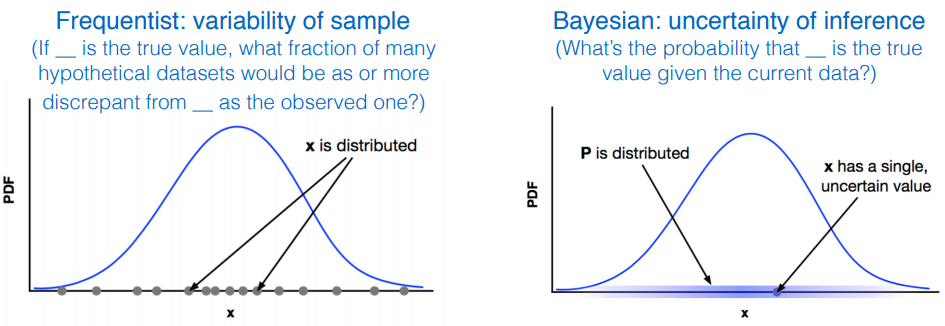
\includegraphics[width=0.7\linewidth]{Figures/freqbaye}
	\caption{Visualised comparison of frequentist and Bayesian results, from \citet{Wolfgang2016} }
	\label{fig:freqbaye}
\end{figure}

A significant problem of the frequentist approach is that its interpretation of result inevitably encourage people to fixate on numerical determinants such as p-value and did not allow for uncertainty. Study such as \citet{open2015estimating} have shown that psychology experiments with frequentist results often have weaker claim to evidence than evidence suggested by p-value from studies, a large proportion of the studies are not repeatable. A p-value of 0.051 and a p-value 0.049 are very similar probability-wise; however, people could deduce significance and non-significance just because 0.049 is lower than the significance level, and 0.051 is not if they fixate on the significance level of 0.05.  Results from Bayesian analyses are less prone to such issue, as it results are in posterior probability distributions, even though a it is harder to interpret, it contains much more information within the posterior probability distribution compares to the frequentist p-values. Secondly, Bayesian inference allows the inclusion of external information from sources other than just the observation; this is a form of evidential probability and allows for sequential learning \citep{baath2015, Jia2018}. For time-series data, the way Bayesian includes information from both the past and present make much more sense than considering only the present observation because datasets with sequential measurements such as time-series data often observe autocorrelation, where information from the past strongly associates with present observations. Also, as mentioned in the previous section, incorporating external information about hospital capacity makes much more sense than the frequentist approach as the primary determining factor for hospital congestion are the capacity it could accommodate. We could observe a very improbable arrival, but if this number still falls under the capacity, there is no congestion. Lastly, Bayesian has an advantage over frequentist for large datasets with complex structures. As models get more complex and more nested, the likelihood for over-fitting, over-parametrisation and multiplicity often increase for simple frequentist models. Bayesian allows utilisations of finer definitions for highly custom models that also penalises over-parametrisation \citep{baath2015, bolker2009generalized, kruschke2015bayesian}.

\subsection{Prior Selection}

The essence of Bayesian inference lies within the Bayes theorem, that is, given prior and likelihood, we can deduce the posterior. A prior probability distribution refers to a probability distribution that expresses ones' prior beliefs about an observation. For example, the prior could be the probability distribution representing the expected patient arrivals at an Emergency Department (ED). There are several acceptable methods of obtaining the prior. Firstly, prior can be determined from past information, such as historical hospital records. Secondly a prior can be a purely subjective opinion from an expert in the field, an ED staff making claims about average patient arrivals also seem reasonable, and lastly statistical principles can be applied to synthesis a prior, a normal distribution is often used for large samples if the prior belief if that the unknown parameter is most likely equal and have few outliers. Also, people often choose to use a conjugate prior to simplifying the calculations of the posterior distribution.

\newpara

Priors can be classified by the amount of information it contains, in terms of informative, weakly informative and non-informative priors. Informative priors define specific information about a variable. Historical information about patient arrivals can be modelled to give predictions, and optimum solutions can be used as the prior. A weakly informative prior contains partial information about a variable, parameters are more vague and rounded but still regularises the parameter estimates reasonably well. A possible standard to distinguish informative and weakly informative prior is that for informative priors, people with different backgrounds are likely to have very different idea about the prior, and for weakly-informative prior, people from different background should agree with the prior. Non-informative priors in another hand, contains no information, such as the use of a uniform or flat line distribution that contain no variation. Informative priors are the proper way to introduce the available informations to the model, and will provide solutions to computational issues and improve efficiency if it was correctly assigned, non informative prior in other hand challenges the notion of prior, but are often thought of as the reference models,and serve as starting point of more informative prior distributions. The weakly informative prior stands as a compromise between two sides \citep{carlin2008bayesian, golchi2016informative}.

\newpara

Parameters of prior distributions are also the hyper-prior because it gives rise to the parameter being estimated. For example, if parameter $\lambda$ of a Poisson distribution is used to model the parameter $\mu$ of a normal distribution, it is then said that $\lambda$ is a hyper-parameter. Hyper-parameters themselves may have hyper-hyper-prior distributions expressing beliefs about their values. Moreover, a Bayesian model with more one level of priors is called a hierarchical Bayesian model.

\subsection{Hierarchical Bayesian models}

\begin{figure}[hb]
	\centering
	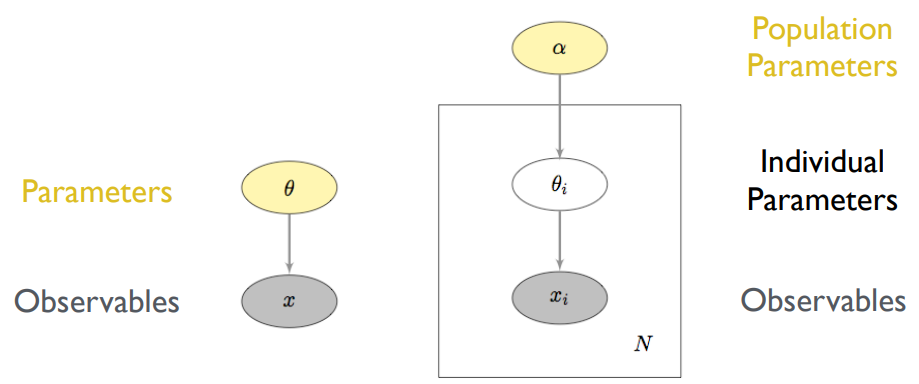
\includegraphics[width=0.7\linewidth]{Figures/hbm}
	\caption{Modelling structure between regular and Hierarchical Bayesian Models, from \citet{Wolfgang2016}}
	\label{fig:hbm}
\end{figure}

Information about the structure of hierarchical data can be processed and utilised with the use of Hierarchical Bayesian Models (HBM). Parameters within the HBMs contain a nested hierarchical structure, which meant that parameters of a higher hierarchy control the parameters of the lower hierarchy. The left plot in figure~\ref{fig:hbm} described the relationship between parameters and observations of an Independent Bayesian Model (IBM), for the case of IBM, observations are directly generated from parameters from a single level probability distributions and thus considered independent. The right plot in figure~\ref{fig:hbm} described the relationship between parameters and observations of an HBM, for the case of HBM, population parameters and observations control individual parameters is generated from a multi-level probability distributions \citep{gelman2007data, Wolfgang2016}, therefore we have this pooling of information, and there is no independence.

\newpara

In Bayesian terms, a simple IBM follows equation~\ref{baye8}, considering only the individual parameter $\theta$ and observations $x$. For an HBM extra population parameter, $\alpha$ can be incorporated and written with the formula shown in equation~\ref{baye9}. 

\begin{equation}\label{baye8}
\begin{aligned}
\overbrace {p(\theta|x)}^{\text{Posterior}} & \propto \overbrace {p(x|\theta)}^{\text{Likelihood}} \overbrace {p(\theta)}^{\text{Prior}} 
\end{aligned}
\end{equation}

\begin{equation}\label{baye9}
\begin{aligned}
\overbrace {p(\alpha,\theta|x)}^{\text{Posterior}} & \propto \overbrace {p(x|\theta,\alpha)p(\theta|\alpha)}^{\text{Likelihood}} \overbrace {p(\alpha)}^{\text{Prior}}
\end{aligned}
\end{equation}

\newpara

for level 1 categories i and level 2 categories $j \in i$, 

\begin{equation}\label{baye9}
\begin{aligned}
x_{ij}|\theta_{ij}&\overset{ind}{\sim}f(.|\theta_{ij})\\
\theta_{ij}|\alpha&\overset{iid}{\sim}f(\alpha)\\
\alpha&\sim f(.)
\end{aligned}
\end{equation}

where $i = 1,...,n,$ and $j = 1,...,n_i,$ and

\begin{equation}\label{baye9}
\begin{aligned}
x_{ij}|\theta_{ij}&\overset{ind}{\sim}f(.|\theta_{ij})\\
\theta_{ij}|\phi_i&\overset{iid}{\sim}f(\theta_{ij}|\phi_i)\\
\phi_i|\alpha&\overset{iid}{\sim}f(\phi_i|\alpha)\\
\alpha&\sim f(.)
\end{aligned}
\end{equation}

The former model is the ‘independence’ model (no pooling), and the latter is the ‘hierarchical’ model (pooling within level 2). 

\newpara

The way HBMs integrate group information with a pooling process is a partial-pooling model that compromise between complete-pooling and no-pooling models. With complete pooling, each unit is assumed to have the same parameter, leaving no independence and therefore contain zero population variance. With no pooling, each unit is assumed to have different and independent parameters, and this complete independence corresponds to infinite population variance. Both complete-pooling and no-pooling models have significant applications in preliminary statistical analyses but unlikely to accommodate real-life data very well; as it is unlikely and does not make sense for scenarios of no independence and complete independence to happen in real-life. For HBMs, individual estimates tend to shrink toward the population mean, and this effectively lowers the overall Root Mean Square Error (RMSE). RMSE is a popular goodness-of-fit value used to measure the difference between real and predicted values during cross-validation analyses. Therefore, there is no surprise that studies have shown that hierarchical models tend to give a better prediction compare to no-pooling and complete-pooling models in all levels \citep{gelman2006multilevel, gelman2007data, park2004bayesian}. 

\subsection{DIC}

In Bayesian statistics, deviance is often used to evaluates the goodness-of-fit statistic for a model. \citet{spiegelhalter2002bayesian} has proposed the idea of using deviance information criterion (DIC) as a tool for goodness-of-fit comparison between Bayesian models. DIC is defined as the expected deviance $\bar{D}$ plus the effective number of parameters in the model $p_D$. 

\begin{equation} \label{DIC}
\begin{aligned}
DIC = \bar{D}+p_D 
\end{aligned}
\end{equation}

which is also equivalent to 

\begin{equation} \label{DIC2}
\begin{aligned}
DIC = D(\bar{\theta}) +2p_D
\end{aligned}
\end{equation}

 where $\bar{\theta}$ is the expectation of $\theta$.
 
 \newpara
 
 DIC can be thought of as an approximation to the deviance, or the out-of-sample predictive error, therefore models with lower DIC are preferable.DIC criterion is particularly useful in Bayesian model selection problems where the posterior distributions of the models have been obtained by Markov chain Monte Carlo (MCMC) simulation. The smaller the DIC, the more accurate the model is for predictions and thus preferred. Model DICs can be generated by using \texttt{dic.samples} function from the \texttt{rjags} package within the R environment, The definition of $p_D$ used by \texttt{dic.samples} function is the one proposed by Plummer (2002).

\subsection{Effective Sample Size}

The idea effective sample size (ESS) is to provide a unit that converts dependent samples into units of independent samples. In other words, the ESS is an estimate of the sample size required to achieve the same level of precision if that sample was a simple random sample. For the case of highly correlated samples, 1,000 samples from a Markov chain can be only equivalent to 100 independent samples. In the case of a weakly correlated sample, 1000 samples from a Markov chain can be only equivalent to 300 independent samples \citep{Cook17, kass1998markov}. The equation for ESS is:

\begin{equation} \label{ESS2}
\begin{aligned}
\mbox{ESS} = \frac{n}{1 + 2\sum_{k=1}^\infty \rho(k)}
\end{aligned}
\end{equation}

Where n is the number of samples and $\rho(k)$ is the correlation at lag $k$.The MCMC process causes the draws to be correlated, as shown in the Markov chain algorithm (equation~\ref{baye6}) the sample from time $t + 1$ depends on the sample from time $t$. This means that the effective sample size is generally lower than the number of draws and is used for calculations. Any Markov chain between 0 ESS and completely ESS is reasonable.

%------------------------------------------------------------------------------------------    

\section{Hierarchical time-series}

\subsection{ Structure of Hierarchical time-series}

A time series refers to a series of data points that are ordered in time and or contain information about when the numbers were recorded \citep{das1994time,hyndman2018forecasting}. Time series analysis is an intriguing part of epidemiology and clinical research because time often has a strong association with the development of diseases and often reflect essential population-level information. Time series in epidemiology and clinical research often can have a hierarchical structure, where many time-series aggregate together to form broader categories of time series by specific population attributes.  Finer International Statistical Classification of Diseases and Related Health Problems (ICD)\citep{WHO2019} categories at a lower level of hierarchy diagnoses can be aggregated into broader categories at a higher hierarchy level. 

\newpara

A hierarchical time series (some time called grouped time series) can be represented with a hierarchical tree diagram. Figure~\ref{fig:treesimple} shows a simple 2 level hierarchical structure. At the very top of the hierarchy, it is the total; it can be calculated by summing of all categories, it represents the sampling population, and can be thought of as the start (level 0) of the hierarchy. The total can be disaggregated into subcategories at level 1 of the hierarchy, and subcategories can be disaggregated into sub-subcategories at level 2 of the hierarchy, and so on. Categories a hierarchy higher can be thought as the parent, and categories a hierarchy lower can be thought as the children of another hierarchy. The observations of the total series given time $t$ is denoted by $y_{total,t}$ for $t=1,2,3…,n$ with $,t$ standing for given time $t$ and $n$ standing for the length of the time period. Additional subscripts should be added for the subsequent levels, for example, $y_{A,t}$ denotes the $t$th observation of series A at level 1 of the hierarchy, $y_{AA,t}$ denotes the $t$th observation of series AA at level 2 of the hierarchy, and so on.

\newpara

For real-life hierarchical time series datasets, lets use occurrence of death in New Zealand as an example, $y_{total,t}$ could be the counts of mortality in intervals of month. We could easily disaggregate our data into geographical subcategories such as North and South island, so at level 1 of the hierarchy we will have $y_{A,t}$ for mortality counts for north island given month, and $y_{B,t}$ mortality counts for South island  given month. 

\begin{figure}[!t]
	\centering
	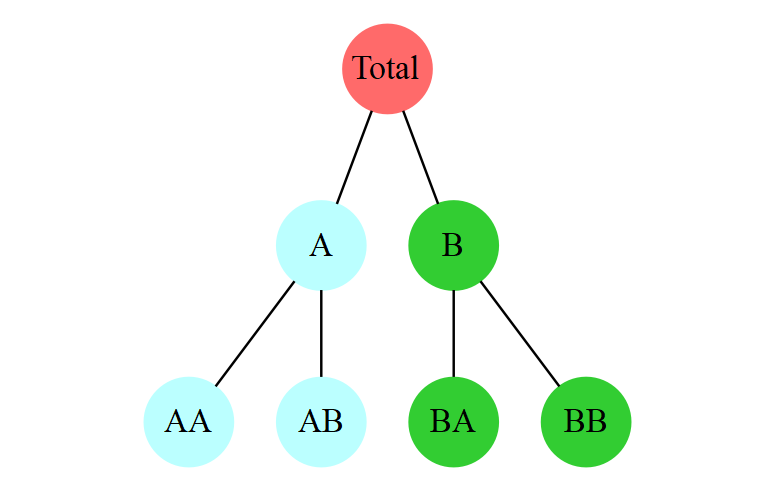
\includegraphics[width=3in]{Figures/treesimple}
	\caption{A 2 level hierarchical structure}
	\label{fig:treesimple}
\end{figure}

\newpara

Hierarchical relationship descripted in figure~\ref{fig:treesimple} can be presented with following equations:

\begin{equation}\label{equ:ts1}
\begin{aligned}
y_{total,t} = y_{A,t}+y_{B,t}
\end{aligned}
\end{equation}

\begin{equation}\label{equ:ts2}
\begin{aligned}
y_{A,t}=y_{AA,t}+y_{AB,t}\quad \quad y_{B,t}=y_{BA,t}+y_{BB,t}
\end{aligned}
\end{equation}

The relation can then be generalised into: , 

\begin{equation}\label{equ:Ts3}
\begin{aligned}
& y_{total,t} = \sum_{i=1}^{n_{i}} y_{i,t} \quad y_{i,t} = \sum_{j=1}^{n_{ij}} y_{ij,t} \quad... \\
\Rightarrow \quad & y_{parent,t} = \sum y_{children,t}
\end{aligned}
\end{equation}

Moreover, this can be thought of as aggregation constraints where observed values from bottom level hierarchies must sum to the observed value of the parent of these values. 


\newpara

Hierarchical time series can also be translated into a $n \times m$ matrix $S$, when $n$ equals to the number of observation of each time series, and when m equal to the total number of categories when considering categories from all levels \citep{Hydnman2016,wickramasuriya2019optimal}. For the hierarchical structure in Figure~\ref{fig:treesimple}, we can write with a matrix formula:
\begin{equation}\label{equ:Ts4}
\begin{aligned}
Y_t  \quad & \quad \quad \quad S \quad \quad \quad \quad b_t \\
\begin{bmatrix}
y_{Total,t} \\
y_{A,t}\\
y_{B,t} \\
y_{AA,t} \\
y_{AB,t}\\
y_{BA,t} \\
y_{BB,t}
\end{bmatrix}
= &
\begin{bmatrix}
1 & 1 & 1 & 1 \\
1 & 1 & 0 & 0 \\
0 & 0 & 1 & 1 \\
1  & 0  & 0  & 0  \\
0  & 1  & 0  & 0  \\
0  & 0  & 1  & 0  \\
0  & 0  & 0  & 1
\end{bmatrix}
\begin{bmatrix}
y_{AA,t} \\
y_{AB,t} \\
y_{BA,t} \\
y_{BB,t}
\end{bmatrix}\\
\end{aligned}
\end{equation}

\subsection{Forecasting approaches}

A classical method for hierarchical forecasting is the \textbf{bottom-up} approach. In this approach,  independent forecasts of each time-series series at the leaf(very bottom) level of the hierarchy are aggregate to workout the forecasts for the upper levels of the hierarchy until reaching the total. The main advantage of the approach is that no information is lost during the whole process; however, modelling and predictions of lower-level time-series often very challenging due to an abundant presence of noise \citep{hyndman2014optimally}. A level one level on top another level can be considered as the parent as it is where the lower level come from, vice versa a level one level below another level can be considered the children.  We can think of the hierarchical relationship, as shown in equation~\ref{equ:Ts5}, where the estimated values from the parent levels are the aggregations of estimates from children levels. 

\begin{equation}\label{equ:Ts5}
\begin{aligned}
\sum y_{children,t} \Rightarrow \quad & y_{parent,t} 
\end{aligned}
\end{equation}

\newpara

Another method for hierarchical forecasting is the \textbf{top-down} approach. In this approach, the forecast of each time-series series at the top level(total) is disaggregated down the hierarchy, with information of the hierarchical structure from historical data. This approach has reduced noise and is easier to model, but some information is lost during the process \citep{hyndman2014optimally}.  We can think of the relationship as shown in equation~\ref{equ:Ts6}, where the estimated values from the children level are comes from the dis-aggregations of estimates from the parent levels, given an estimation of a hierarchical structure $H$. 

\begin{equation}\label{equ:Ts6}
\begin{aligned}
\quad & y_{parent,t} | H \Rightarrow \sum y_{children,t} 
\end{aligned}
\end{equation}

\begin{figure}[!h]
	\centering
	\subfloat[Top down]{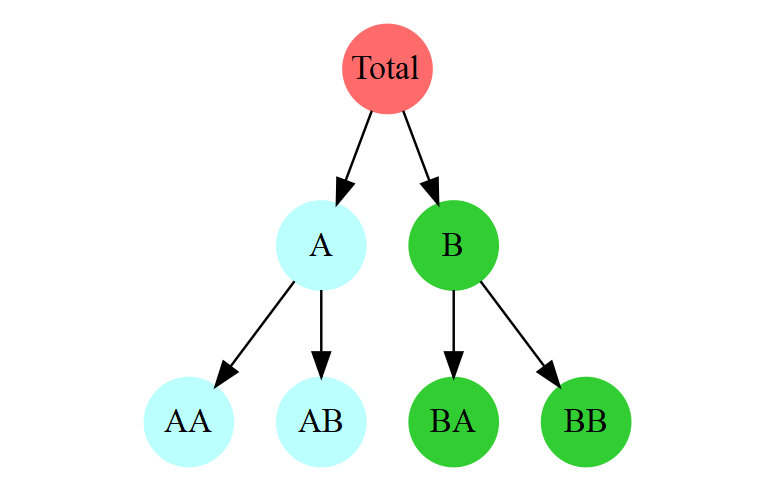
\includegraphics[width = 2in]{Figures/topdown}} 
	\subfloat[Bottom up]{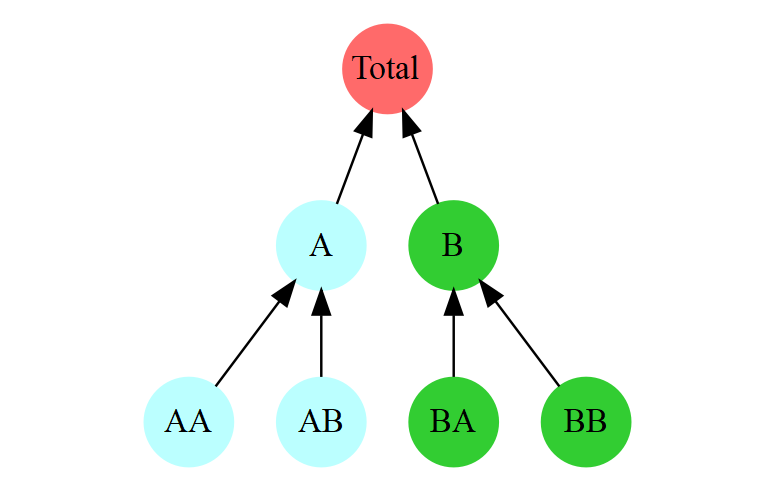
\includegraphics[width = 2in]{Figures/bottomup}}
	\subfloat[Optimum reconciliation]{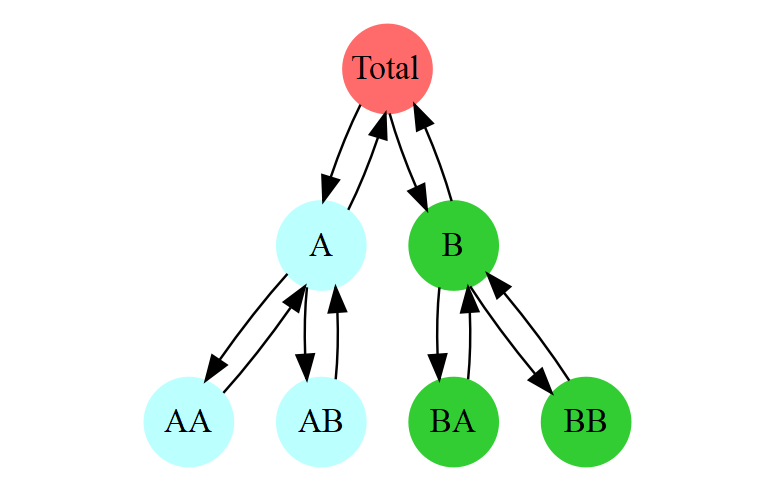
\includegraphics[width = 2in]{Figures/optim}}\\
	\caption{Top-down, Bottom up and Optimum reconciliation approach}
	\label{fig:approaches}
\end{figure}

\newpara 

\cite{hyndman2011optimal} recommend a new method of \textbf{optimal reconciliation} for the forecast of hierarchical time series data for its feature and performance. The optimal reconciliation works by independently forecasting each time-series at all levels of the hierarchy, and then reconcile each forecast with regression models by minimising the forecasting error (Figure~\ref{fig:approaches}). The most significant advantage the optimal reconciliation approach is that all of the information available within each level of the hierarchical structure are in consideration during the forecasting process. The idea is that important information may lye within any particular level within the whole hierarchical structure, and can be hard to detect from other levels if we only consider one level at the time \citep{hyndman2018forecasting}. A weakness of the optimal reconciliation is that even if the observations considered are natural numbers; it could still produce negative predictions that are the optimum solution to the prediction but does not make sense in real-life. In many instances, time-series predictions need a set of non-negative reconciled forecasts. If the demand for a particular commodity for the time-period $t = 2020$ is $-5$, it does not have any sense at all. 

\newpara

Time-series forecast with all approached mentioned above can be made by using the \texttt{forecast()} function with an \texttt{hts} object (created using \texttt{ts} and \texttt{hts} function)in under the \texttt{hts} package \citep {hts} in the R environment. Optimal non-negative reconciled forecasts are currently not available for the \texttt{hts} package within the R environment, but a little bird told me \texttt{hts} package with non-negative reconciled forecasts will be updated at the end of July 2019. For another note, optimum reconciliation forecasts used for the next session does have negative values, but the values are mostly extremely small so they are treated as 0 values. 



%------------------------------------------------------------------------------------------
\newpage
\section{Outline of Thesis}

The organisation of the thesis is described in the follows: 

\newpara

\ding{169} \textbf{\Cref{chap:Background}} starts with the introduction of examples of where these issues in hierarchical structure arise; these include background and concepts of the topics, including emergency department congestion and anomaly detection. Technical background about statistical methods and techniques necessary for our methods, these include topics of and within Bayesian inference and hierarchical time-series predictions. Lastly, we included outlines for the thesis and notations and conventions for this thesis. 

\newpara

\ding{169} \textbf{\Cref{chap:Simulations}} presents methods, results and discussion of our simulation studies of anomaly detection in several settings. The first simulation looks on how different priors would affect the goodness of fit and posterior results of Independent Bayesian Models(IBM). The second simulation compares scenarios with different increments of anomalies added. The third simulation compares scenarios with different different branching at Category A, with addition of a constant anomaly.

\newpara

\ding{169} \textbf{\Cref{chap:MIMIC}} presents methods, results and discussion of our studies of anomaly detection with MIMIC-III, a publicly-available database with health-related data. More specifically, for four scenarios which include original observations and observations with anomalies added on categories of common, rare and extremely rare disease diagnoses. 

\newpara

\ding{169} \textbf{\Cref{chap:Conclusion1}} provides a final conclusion and overview of studies presented in this thesis.

\newpara

\begin{itemize}
	\item  \textbf{The Appendix} includes:
	\begin{itemize}
		\item  Descriptions of custom R function created, and R code used to implement different prior models, Independent Bayesian Model and Hierarchical Bayesian Model, used in \Cref{chap:Simulations} and \Cref{chap:MIMIC}.
	\end{itemize}
\end{itemize}

%------------------------------------------------------------------------------------------
\newpage
\section{Notations and conventions}

The following notation and conventions are used throughout this thesis to aid\\ readability:

\newpara

\begin{tabular}{rl}
	\textbf{Software} & Software is denoted by mono-space font with boldface.\\
	& For example: This plot is created using \texttt{\textbf{R}} codes. \\
	
	&\\ 
	
	\textbf{R packages} & Package names are given in mono-space font .\\
	& For example: This function is from the \texttt{GOpro} package. \\
	
	&\\ 
	
	\textbf{R functions} & Functions are denoted with mono-space font with two trailing \\
	& parentheses. Arguments are similarly displayed in monospace \\
	& with format "value" or "argument = value".\\
	& For example: This plot is created using \texttt{ggplot()} function.\\
	& For example: We used \texttt{dnorm(1, sd = 0.1) as our hyper-prior} \\
	
	&\\ 
	
	\textbf{Quotes} & Direct quotes should be denoted using Italic font\\
	& For example: "\textit{Shall I compare thee to a summer’s day}" \\
	
	&\\
	
	\textbf{Textbooks} & Text book and journal titles should be denoted using Italic font\\
	& For example: "\textit{High Performance Computing for Disease Surveillance}" \\
	
	&\\
	
	\textbf{Key words} & Some key words are denoted in bold font\\
	& For example: We have \textbf{significant} results.  \\
	
\end{tabular}